
\begin{center}\texttt{3 - BRUF, Big Requirements Up Front}\end{center}
\hrulefill \\

\noindent Command-and-Control, the traditional, much more formal approach.

\noindent Project def.: a project is a temporary endeavor undertaken to create a unique product, service, or result. $\rightarrow$ there's a beginning and an end to the prj; 

\noindent Planning is required, you want to plan each activity of the prj;

\noindent The time span to carry out the project is predefined: after that, either you're done or you're not done;

\noindent Several specialisms are involved, typically -  many different people with different expertise are required;

\noindent The working groups are temporary and relative to this one project's timespan;

\noindent The workflow is divided into Phases;

\noindent Resources are constrained - no infinite time or money or office space. Resources are limited, thus the usage needs to be planned;

\noindent Motivations for starting a prj (influences the way the prj will be structured, helps define more accurate Requirements). Could be one or more:
\begin{itemize}
    \item market demand: there could be the need for this product;
    \item strategic opportunity/business need: you want to enter that market;
    \item social need;
    \item environmental consideration;
    \item customer request;
    \item technological advance;
    \item legal requirement.
\end{itemize}

\noindent Project Management is the application of knowledge, skills, tools, and techniques to project activities to meet the project requirements. Helps companies deliver a product efficiently and effectively. 

\noindent Macro groups of activities of PM:
\begin{itemize}
    \item initiating;
    \item planning (expensive!!!);
    \item executing;
    \item monitoring and controlling (is what we did in line with the plan? if not, correct the execution);
    \item closing.
\end{itemize}
\begin{figure} [H]
    \centering
    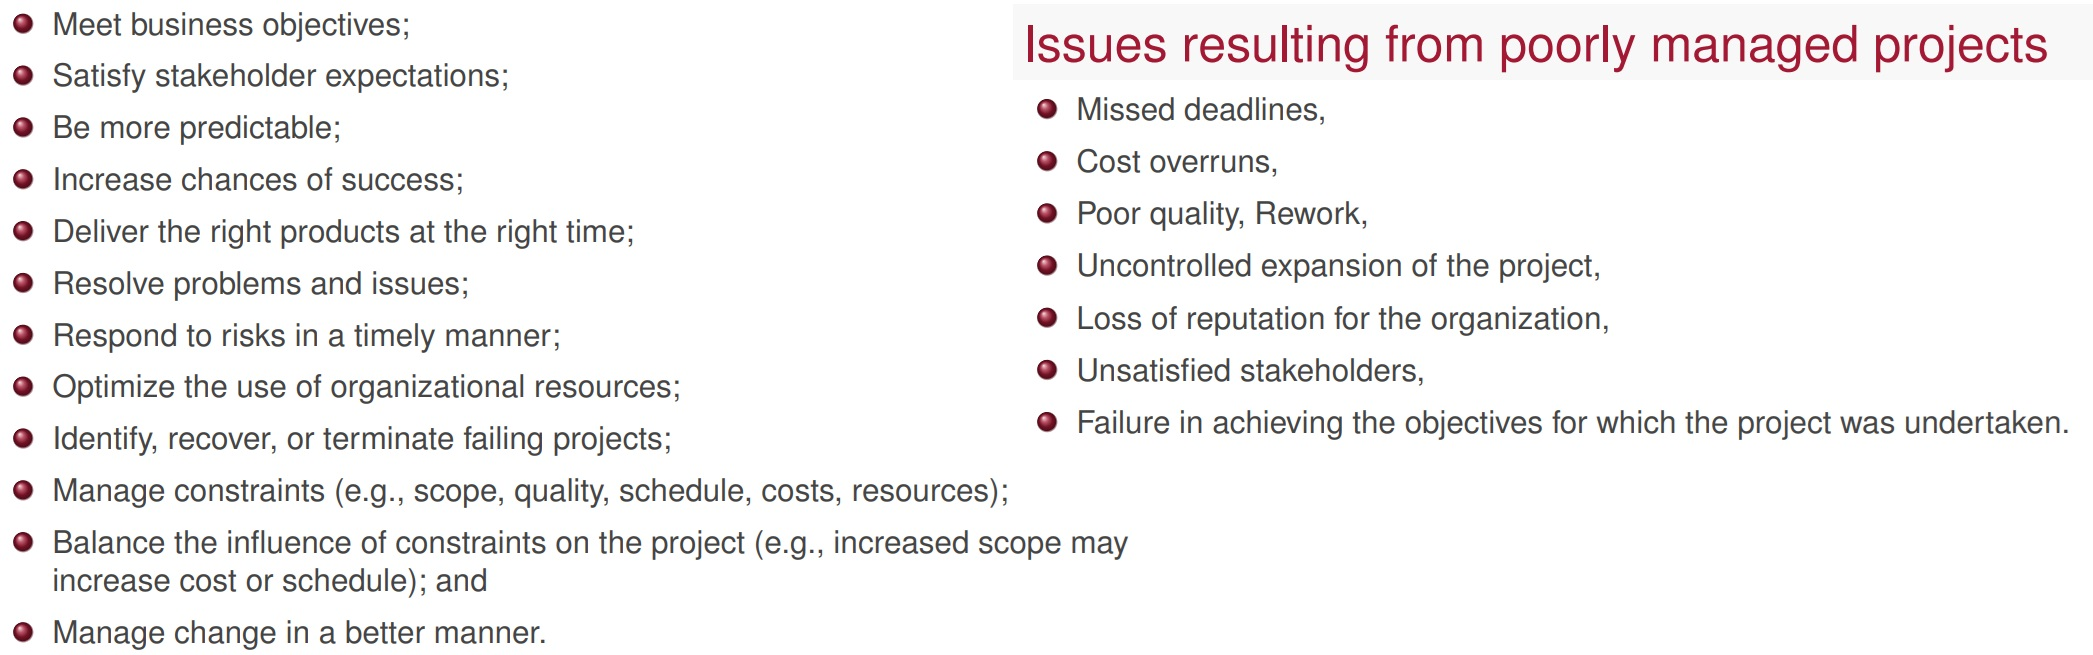
\includegraphics[scale=0.42]{Figures/03/benefit_issues.jpg}
    \caption{Benefits of good project mgmt VS. consequences of poor project mgmt}
    \label{fig:pmbi}
\end{figure}
\noindent 10 Knowledge Areas you need to acquire if you want to become a Project Manager:
\begin{itemize}
    \item Prj Integration Mgmt: coordination among all processes and activities. A process to manage processes. Meta :D
    \item P. Scope M.: ensuring that the project includes all and only the activities required to complete the prj (the best m.o. is to rely on past experience);
    \item P. Schedule M.: techniques to organize the timing of the prj, taking dependencies into consideration for example;
    \item P. Cost M.: money! estimation of the costs of the prj, and how to sustain the costs over time (cash flow);
    \item P. Quality M.: perform activities to control the quality of the prj and the product (even testing);
    \item P. Resource M.: identify the resources, acquire and manage those you have and don't have;
    \item P. Communications M.: all things spread-prj-information adequately. Gather, spread, deliver, yadayada, information;
    \item P. Risk M.: identify, analyze, respond to, monitor, risk factors! i.e., uncertainties, elements beyond control;
    \item P. Procurement M.: acquiring things? Buying, hiring, HR stuff;
    \item P. Stakeholder M.: identifying the people, analyze sh expectations and so on, all things SHs;
\end{itemize}

\noindent The Prj Manager is the one person assigned by the corporation to lead the team through the project. They are responsible for achieving the goals. They have leadership, team building skills, they are motivators, great communicators and persuaders. Decision making, political and cultural awareness, negotiation, conflict mgmt, coaching and recognizing people's improvements are some more skills required for a good PM.

\noindent Software Prj Management is a peculiar engineering discipline bc software is intangible, thus it costs less wrt its complexity, plus the context is constantly and quickly evolving, and because it's ethereal it's easy to change (which is a double edged sword).\\

\noindent on Feasibility:

\noindent The goal is to answer questions such as: is it worth to start this project? Identify business case and analyze the market and mk strategies; the accuracy of the analysis will not be great at this stage.  Building a small prototype might help with that. As a developer, you might be working for an external customer (you are the contractor, i.e. under contract), or you're dev'ing a product for your own company, the difference might influence the study. Do we build or do we buy, for example? Are we deriving a project to answer a call, i.e. by the EU?


\noindent Feasibility study: document reporting the effort of feasibility, contains all that you gathered to provide answer to said questions, though in a somewhat general way. Revenue estimation, risks, market analysis, benefits, operational infrastructure, general implementation plan, management plan. If the answer is yes, it's worth, you'll proceed with the detailed planning.

\noindent on Project Planning: phase in which we derive a detailed plan. The best plan you can think of to derive the prj. Consider the prj objectives as post-conditions of the process, things you want to get done by the end. They should be: specific (well defined), measurable, achievable, relevant, time-constrained (you can do it in the time at your disposal).

\noindent Step-Wise Method management methodology - to derive a schedule.
\begin{enumerate}
    \item [0] Select a Project: in most cases you have many projects to choose from, so you do Project Portfolio Management (portfolio being a collection of programs and prjs): give an overview of the possible projects and prioritize those who should be accepted;
    \item [1] Identify Scope and Objectives: and the governance, thus a project authority and a Prj Mgmt Board (PMB), and one Manager for sure; identify the stakeholder, define the objectives as best as you can;
    \item [2] Identify prj infrastructure: people involved and the activities they will perform, following which procedures, how the team will exchange information;
    \item [3] Analyze prj characteristics: understand how to perform activities based on what kind of prj you have in hand - is it safety critical? Gather the right people for that. Select a methodology and life cycle approach: prototyping, iterative, incremental...; estimate the resources;
    \item [4] Identify prj product and activities: organize the work; maybe deliver some intermediate artefacts, derive the PBS, product breakdown structure, i.e. breaking down the system into components to better organize the work (architecture oriented). Produce the PFD, Product Flow Diagram for generic product flows, whatever that means; Produce the ideal activity network: dependency graph between activities (do this before you do that, if no dependencies you can run in parallel! not considering the resources available yet, you will introduce those and adjust the plan later);
    \item [5] estimate effort for each activity: understand how much time and resources you need for each activity, trying to find a good balance between time and people investment;
    \item [6] identify risks: things will very likely not go as planned. how will we adjust the plan if something goes awry or any differently?
    \item [7] identify and allocate resources: rooms, names, revise the plans again to adapt to resource constraints;
    \item [8] share this plan you just cooked, with the rest of the team;
\end{enumerate}
This step-by-step procedure is often iterative.

\noindent Cost-benefit analysis:
\begin{itemize}
    \item net profit: diff between total costs and total income over the life of the project (G = R - S);
    \item payback period: time taken to pay back the initial investment (time until break-even point);
    \item RoI: ratio at which you are repaying the investment:
    \[ROI = \dfrac{avgYearlyProfit}{totalInvestment} \times 100 \]
    \item NPV, Net Present Value: given a discount rate $r$, how much money will I get considering at time t the fluctuations of the market and currencies:
    \[NPV = \frac{ValueInYear \times t}{(1+r)^t}\]
    or something
    \item Internal Rate of Return: rate at which it is not worthwhile to invest elsewhere, IRR is a discount rate that makes the net present value (NPV) of all cash flows equal to zero.
\end{itemize}

\noindent Portfolio management and prj choice is a complex business, there are very many and different aspects to consider to make the best choice.

\newpage \underline{Scope,} Objectives and Infrastructures\\

\noindent Organizational context: once you identified the stakeholders for the prj (make sure not to leave out any or there will be trouble!), you will organize the team for the prj. You must put together a team that fits with the operational context, i.e. everything else happening in the company. The PM will interact with the company environment to set up the team and the prj. Companies are organized in different topologies, some being:
\begin{itemize}
    \item Matrix Org:
    \begin{itemize}
    \item Weak Matrix Organization: below the CEO are functional units (with a certain AoExpertise), supervised by a functional manager. The prj team will be a row of such matrix, with members from different Functional units; the team will coordinate with functional managers too, though FMs are not PCoordinators here;
    \item Balanced Matrix Org.: one of the team members from one FU is the PM;
    \item Strong Matrix: there is a PM which belongs to the Project Managers Functional Unit, supervised by the meta manager :D 
    \end{itemize}
    \item Projectized Org: instead of having functional units, the org has project managers under the CEO, and each PM manages a team which works on a project. Coordination happens within said branch. No intermediaries, CEO - PM - Team;
\end{itemize}

\noindent Different org. layouts entail different levels of communication: typically we have inside-prj communication and outside-prj comm., with people who are relevant; as a PM, you want to be capable to communicate with both sides.

\noindent Stakeholders and their engagement is to be carefully managed by the PM: process includes identify, plan mgmt, manage engagement, control engagement. After identifying the people, you want to build a grid that helps the management of SHs: group the stakeholders according to their power (knowledge/authority) and interests (in a XY graph!), or an influence/impact grid, or a salience model. Engagement analysis is about how much SHs can be involved WRT to our goals: some are unaware of the project, some are aware but unwilling to participate (problem), some are neutral, some are supportive, some have a leading interest.

\newpage \underline{Prj Planning} and activities

\noindent Schedule the activities! In different approaches - typically oriented towards the completion of intermediate products that you want to deliver (``deliverables'').\\
A possible approach is the PBS - Product Breakdown Structure: try to identify sub-products that I need to assemble the final product, kind of a divide-et-impera approach. Once I have these macro activities identified, I need to define a Flow, how the intermediate artefact flow between the activities (what dependencies are there?) $\rightarrow$ generate an Ideal Activity Network, direct acyclic graph representing dependencies between activities, to identify a critical path, a SEQUENCE of activities that has the LONGEST duration - that's especially important because it determines the duration of the project. Each activity has a duration, the chain of activities is basically the overall duration ofc.

\noindent How to schedule activities: a simple diagram to represent activities is the Gantt chart - how to derive that Gantt for the project, we're going to see.

\noindent Identify the activities; for each activity, define a start and an end, ensure the resources (human and non) for those activities are available in that time!; then, you can derive a plan, from which plan you can derive a timed cash flow forecast, i.e. when you have to pay things, pretty much, an expense forecast. Once you have a plan, you can notice if there's a drift from said plan in the actualization, so that you can replan and derive a new one.

\noindent Goals of a detailed planning: Feasibility assessment; Resource allocation; Detailed costs for the project upfront; Clarify the motivation of the prj and cooperation among different departments. Deriving the plan is typically an iterative process, you want to harmonize the plan continuously to potentially changing needs. The ultimate goal of planning is to shorten the prj duration - whenever you can, for example, you do that by putting activities in parallel.

\noindent Different strats start from different assumptions and have different objectives: the assumption of CPM is that it has no initial risk associated, it doesn't take risk into account. Bad in the case of complex projects! So basically the CPM is a happy path, the path in which everything goes according to plan - or hope lol

\noindent CPM: we have activities, duration, dependencies. We'll derive a network: begin with a node that corresponds to Day 0, the start of the project, the very first thing; and we also have a Finish node, the day when everything will be finished. In between, we have nodes which look like this: 

\begin{figure} [H]
    \centering
    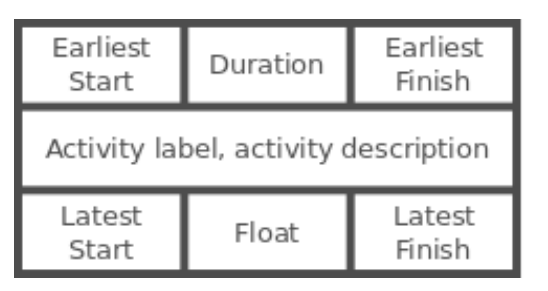
\includegraphics[scale=0.5]{Figures/03/cpm00.png}
    \caption{Intermediate node in the cpm tree.}
    \label{fig:cpmnode}
\end{figure}

\noindent Duration: once you reach the node, you will stay there for the duration specified here. Then the outgoing arcs will be enabled (traversing those has no duration);

\noindent An activity can start only when all the incoming arcs are enabled! There must be no loops, otherwise the project is considered to have potentially infinite duration. No dangling activities, no activity that ends nowhere, there must be an outgoing arc (except the end node I suppose).

\noindent Consider the prj consisting in these activities:

\begin{figure} [H]
    \centering
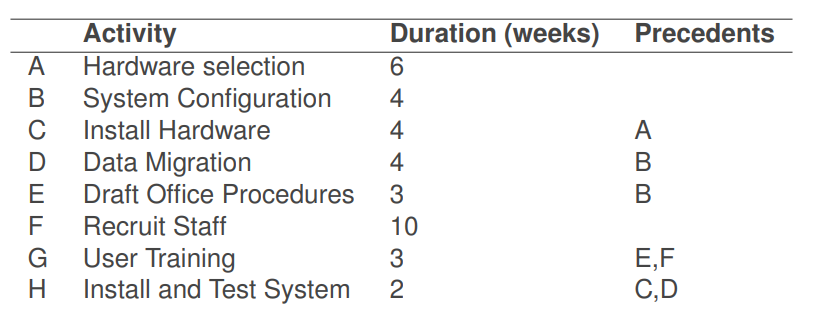
\includegraphics[scale=0.7]{Figures/03/cpm01.png}
    \caption{Precedents is basically another word for Dependencies.}
    \label{fig:cpm01}
\end{figure}

\noindent We can see that nodes A, B and F have no precedents, thus we can immediately start them all. Then we add the ``child'' activities, i.e. those that can start after those 3 are completed. We'll have C, D, and E (not G, cause G also needs E to be done). Add duration for C, D and E. Graph now looks like this:

\begin{figure} [H]
    \centering
    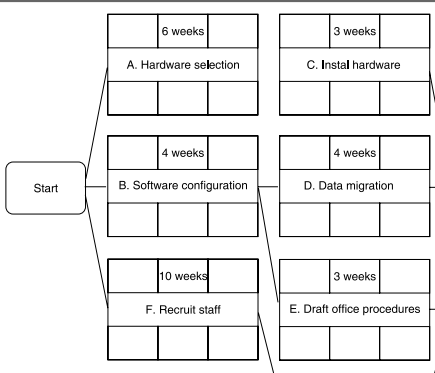
\includegraphics[scale=0.7]{Figures/03/cpm02.png}
    \label{fig:cpm02}
\end{figure}

\noindent Now I can consider H and G, all their dependencies are in the network. Dangling nodes are resolved by sending them into what we might consider their completion activity, i.e. A goes into C, first you select the hardware then you install it:

\begin{figure} [H]
    \centering
    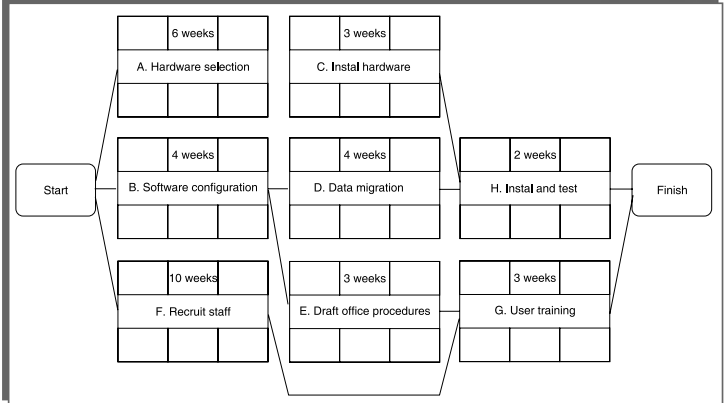
\includegraphics[scale=0.7]{Figures/03/cpm03.png}
    \label{fig:cpm03}
\end{figure}

Now that we have a network, we perform the forward pass (calculate the earliest dates of activities start and prj completion): understand when each activity will start and when they will end, incrementally. Identify the earliest start: date by which the activity can start, the first useful date according to dependencies: A, B and F can start at 0. Earliest end is given by earliest start + Duration. Following the dependency tree, we fill the other cells: the earliest start for C is the earliest end for A. Now onto H: the earliest start for H is the MAX of all the incoming activities' earliest end.

\noindent The duration of the project is the MAX Earliest end at the end of the FWD pass.

\noindent Backward Pass, for additional useful info (the \textit{latest} possible start dates that will not cause a delay): for each node, we can calculate the latest date at which each activity may be started and finished without delaying the end date of the project (in the example, the whole prj takes 13 weeks):  the latest completion date for activities G and H is assumed to be week 13, so activity H must start at week 11 at the latest (13 – 2) and the latest start date for activity G is week 10 (13 – 3). The latest completion date for activities C and D is the latest date at which activity H must start – that is, week 11. They therefore have latest start dates of week 8 (11 – 3) and week 7 (11 – 4) respectively.

\noindent Float: The difference between earliest start date and its latest start date (or, equally, between its earliest and latest finish dates) -  how much the start or completion of an activity may be delayed without affecting the end date of the project. Mind that the total float can be used only linearly! If A uses $n$ float, C will have $n$ less float than originally estimated. Though there might be a \textit{free float} in some situations.

\noindent Once we obtain the critical path and its duration, you can reason on possible optimizations - to do that, you can look at the activities which affect the duration of the project, i.e. those on the critical path: Start - F - G - End. Those which impose the duration of the project, i.e. those that have 0 float (there will always exist one), the PM should keep that in mind and make sure that there are no bumps on the road of the critical path. You might split, for example, F in $F_1$ and $F_2$ in such a way that they have no dependencies, so they can be put in parallel! That way the critical path will be revised. Note that often times you will have more than one possible critical path in the same graph, adding to the complexity.\\

\noindent On Duration: all activities have an optimal allocation of people (as in human resources working on it), it's not like you can reduce time-to-complete as much as you want by shoving many and many more guys on the task. It doesn't scale linearly indefinitely. $\rightarrow$ Effort: the Duration is X assuming the deployment of this many workers of this type. Ten hours is the time it will take if we allocate 20 SDs and 10 JDs on the task. This is resource management, basically, and how they influence the time to completion. If you don't have enough resources, you're gonna have to hire people in, or take more time. It's up to the PM.\\

\noindent An alternative to CPM: arrow based approach. Instead of using nodes. Nodes represent points in time, i.e. they have duration 0, but the arcs are labeled with activities and their duration (not in the picture but oh well, they have duration, the arrow not the nodes). Every node tells you what activities have been completed til then. In case of dangling nodes, you must add a dummy arc (0 Duration 0 Activity) that connects the illegitimate leaf node to the actual end of the graph.
\begin{figure} [H]
    \centering
    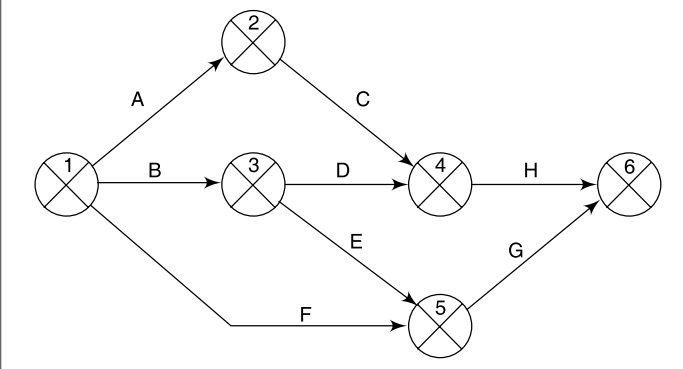
\includegraphics[width=0.75\linewidth]{Figures//03/cpm_arrow.png}
    \label{fig:cpmarrow}
\end{figure}
\noindent Dummy activities are also used in the case of paths with a common node but different behaviour:

\begin{figure} [H]
    \centering
    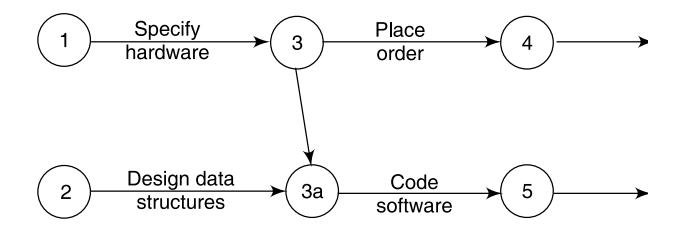
\includegraphics[width=0.5\linewidth]{Figures//03/cpmdummy2.png}
\end{figure}

\noindent BWP, FWP and CP are computed like this:
\begin{figure} [H]
    \centering
    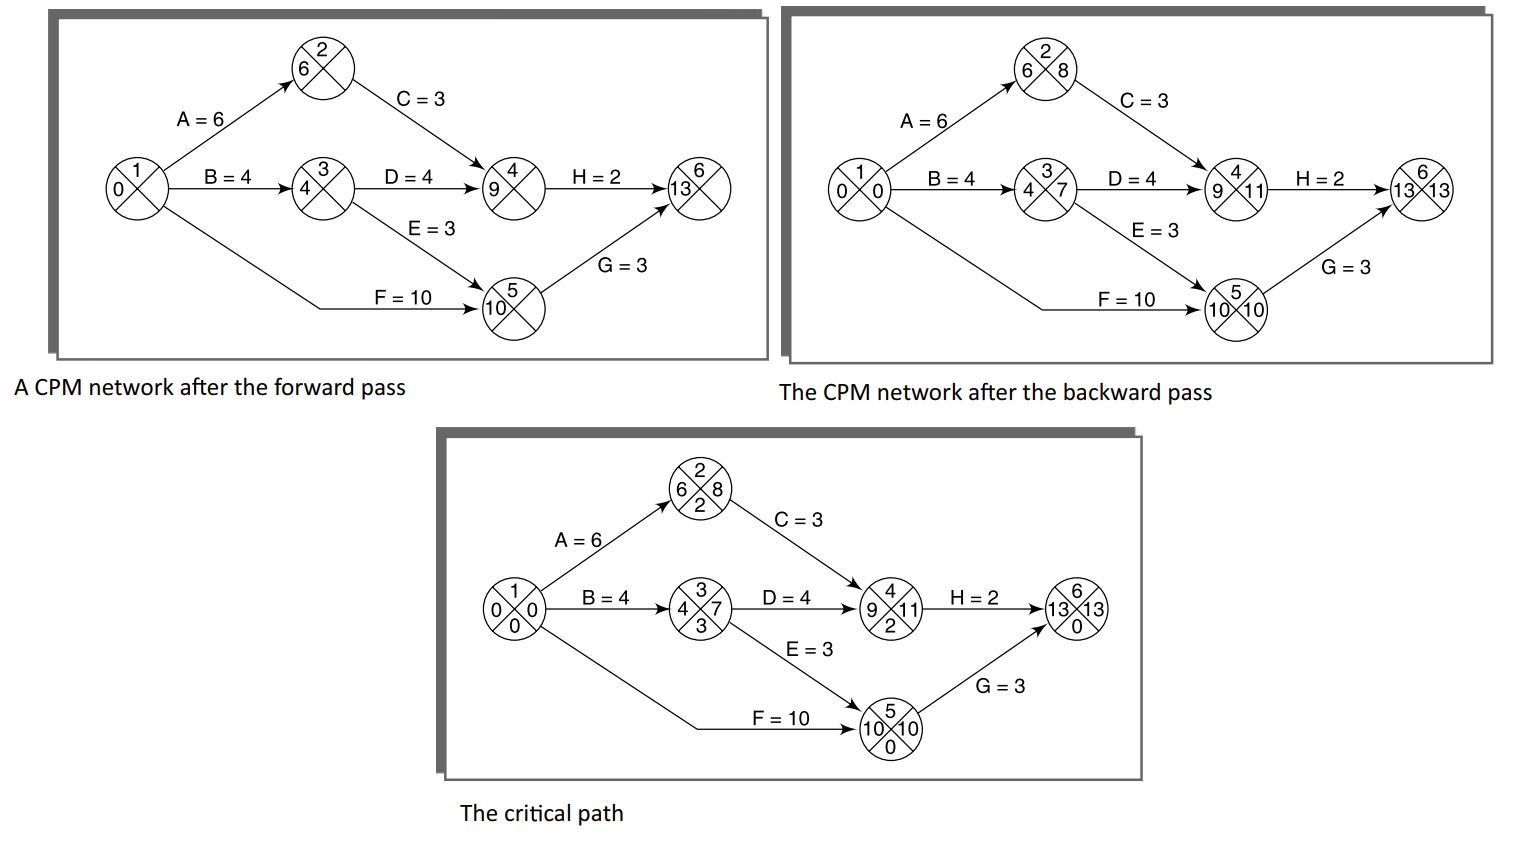
\includegraphics[width=0.75\linewidth]{Figures//03/cpm_arrow_cp.png}
\end{figure}

\noindent Defining activities: apply more than one technique to derive activities and rely on your experience.
\noindent Start from the whole picture and proceed divide-et-impera, decompose it iteratively in subtasks:
\begin{itemize}
	\item WBS: decompose considering the Work perspective;
	\item RBS: decompose considering the Requirements.
\end{itemize}

\noindent Maybe you want to reason on the architecture of the prj, identify the components of the system (for each component, identify activities). As you do this, you get information useful for later monitoring!

\noindent Splitting activities: product-based, identify subcomponents; activity-based, which activities I need to implement the system. Most times it's a hybrid approach. Activities lead to artefacts, from artefacts I get a good map of dependencies. In UP especially, you need those intermediate artefacts!

\noindent How to tell if the activities we derived are complete and adequate? No algorithm to assess that. But you can analyze, upon identifying activities, whether the work is complete:
\begin{itemize}
	\item Can I \textit{measure} status and completion of an activity? If not, then the activity is probably not well defined. Best way is usually to have a deliverable (an artefact that you can deliver);
	\item What about the \textit{duration}, is the activity bounded? If assessing the duration is unclear (6 days to one month?), then you want to define it better;
	\item Does it have a \textit{deliverable}?
	\item Can I estimate time and cost of it? 
	\item Does the duration have an acceptable limit? 2-3 months would be no bueno, reconsider the activity, maybe split it in more activities. They are risky for monitoring! You can discover bad surprises earlier;
	\item Are work assignments \textit{independent}? If not, they might just be one activity instead of many, or they are strongly dependent which is dangerous.
\end{itemize}

\noindent How to identify duration? That too strongly depends on experience. But in general that strongly depends on Effort - more workers, less time to complete (not scalable forever though!). Best effort to move a chair from room A to room B is 2 people, no more, no less. Plus, there's only so much time you can save.

\noindent Techniques to estimate duration of a task:
\begin{itemize}
	\item find similarity with another task: if the durations are much apart, something's off;
	\item historical data: past experience, tangible;
	\item expert advice;
	\item delphi techniques: collaborative approach with experts, they propose evaluation and the team might discuss if they disagree, argument;
	\item three-point technique: to derive a plan. With perception of Risk!! We don't ask the experts the durations, we ask three things: optimal duration, expected duration, pessimistic one. You will then apply a weighted average of the three;
	\item wideband delphi technique: for each of the three points, we discuss! (it's a mix of both)
\end{itemize}


\newpage
\noindent \underline{Resource Allocation}
%VAMOS VAMOSSSSS
\noindent To keep track of the resource usage, you typically have a calendar for each resource (e.g.: a room, a car, a desk). From that, comes a cost schedule, i.e. when I have to pay things! Mostly human resources. 

\noindent Types of resources include: labour (people working on something); equipment (even desks and stuff); materials to be consumed; work spaces; services (e.g.: confcall services); time; money, meta-resource :DD!

\noindent Suppose an activity has duration 20 days, and requires a consultant for 3 Days, Developers for 60 days... but each of the 3 Developers has a calendar with available days. Activity will start at day 50, thus will end at day 70, and has 20 float (day 90): you have to allocate 60 days worth of developers which can be allocated all together in those 20+20 days between 50 and 90.

\noindent Critical Path is often given by the resource availability more than the activity plan per se. Unavailability of resources may use up all the float, or even go overfloat. 

\noindent Assuming all 3 Devs are always available during activity period $(50\div70)$ and considering granularity no thinner than a whole day, the easy solution is $60\div3=20$ they all work in those 20 days and we cover 60 Hr.

\noindent When allocating human resources in particular, try to avoid discontinuity as much as possible - working on and off on a project is really counterproductive. Upon optimization, you can save on the amount of people involved (main objective really). Sacrifice some float, tighten the schedule, but hire way less people. You shouldn't even want a big float anyway.

\noindent Mgmt will ask you to allocate resources in blocks rather than on and off - small gaps are difficult to manage. If you free up a chunk of days for a dev, you can assign the guy somewhere else! Or else ehh, it's a crazy mess very poorly optimized. Company will charge for the gaps as well!

\noindent Optimization techniques:
\begin{itemize}
    \item reduce max number of resource usage (less recruiting people! that also takes time to interviewing and training, rlly bad);
    \item reduce idle time of resources, no gaps;
    \item reduce context switch for HRes;
    \item consider revisiting activities themselves. Splitting them up, most likely.
\end{itemize}

\noindent Once you have resource schedule, you can derive a cost schedule. To some costs, you will apply a constant. Yada yada, you will also define a cash flow, once you know how much this and that costs, you can also tell how much you'll have to pay when.

\noindent 